\documentclass{article}
\usepackage[english]{babel}
\usepackage[utf8]{inputenc}
\usepackage{fancyhdr}
\usepackage[top=1.25in, bottom=1.25in, right=1in, left=1in]{geometry}
\usepackage{graphicx}
\usepackage{filecontents}
\usepackage{amsmath,amsfonts,amssymb,amsthm}
\usepackage{mathtools}
\usepackage{commath}
\usepackage{gauss}
\usepackage{enumerate}

\usepackage{etoolbox}
\makeatletter
\patchcmd\g@matrix
 {\vbox\bgroup}
 {\vbox\bgroup\normalbaselines}% restore the standard baselineskip
 {}{}
\makeatother

\pagestyle{fancy}
\fancyhf{}
\rhead{Introduction to Data Science}
\lhead{Predicting Electricity Spot Price}
\rfoot{Page \thepage}
\makeatletter
\renewcommand{\@seccntformat}[1]{}
\makeatother 

%% Theorems etc. %%%%%%%%%%%%%%
%\swapnumbers
\numberwithin{equation}{section}

\makeatletter
\let\c@equation\c@subsection
\makeatother

\title{%
	Predicting Electricity Spot Price\\
	\large Introduction to Data Science Course Project}
\author{Ville Pirsto, Emil Tigerstedt, Ahsan Abbas}

\begin{document}

% Titlepage separately
\begin{titlepage}
	\maketitle
	\thispagestyle{empty}
\end{titlepage}

\tableofcontents
\clearpage

% ---- Introduction ----
\section{Introduction}
This is the introduction that should contain some pretty general stuff. Below, some initial suggestions are listed.
\begin{itemize}
	\item What was done?
	\item Why? Motivation (canvas)
	\item How? 
	\item Summary of the results
\end{itemize}

% ---- Canvas ----
\section{Project Work Canvas}
\textbf{Note: this is just the canvas template, to be replaced with our filled canvas.}
\begin{figure}[htb]
	\centering
	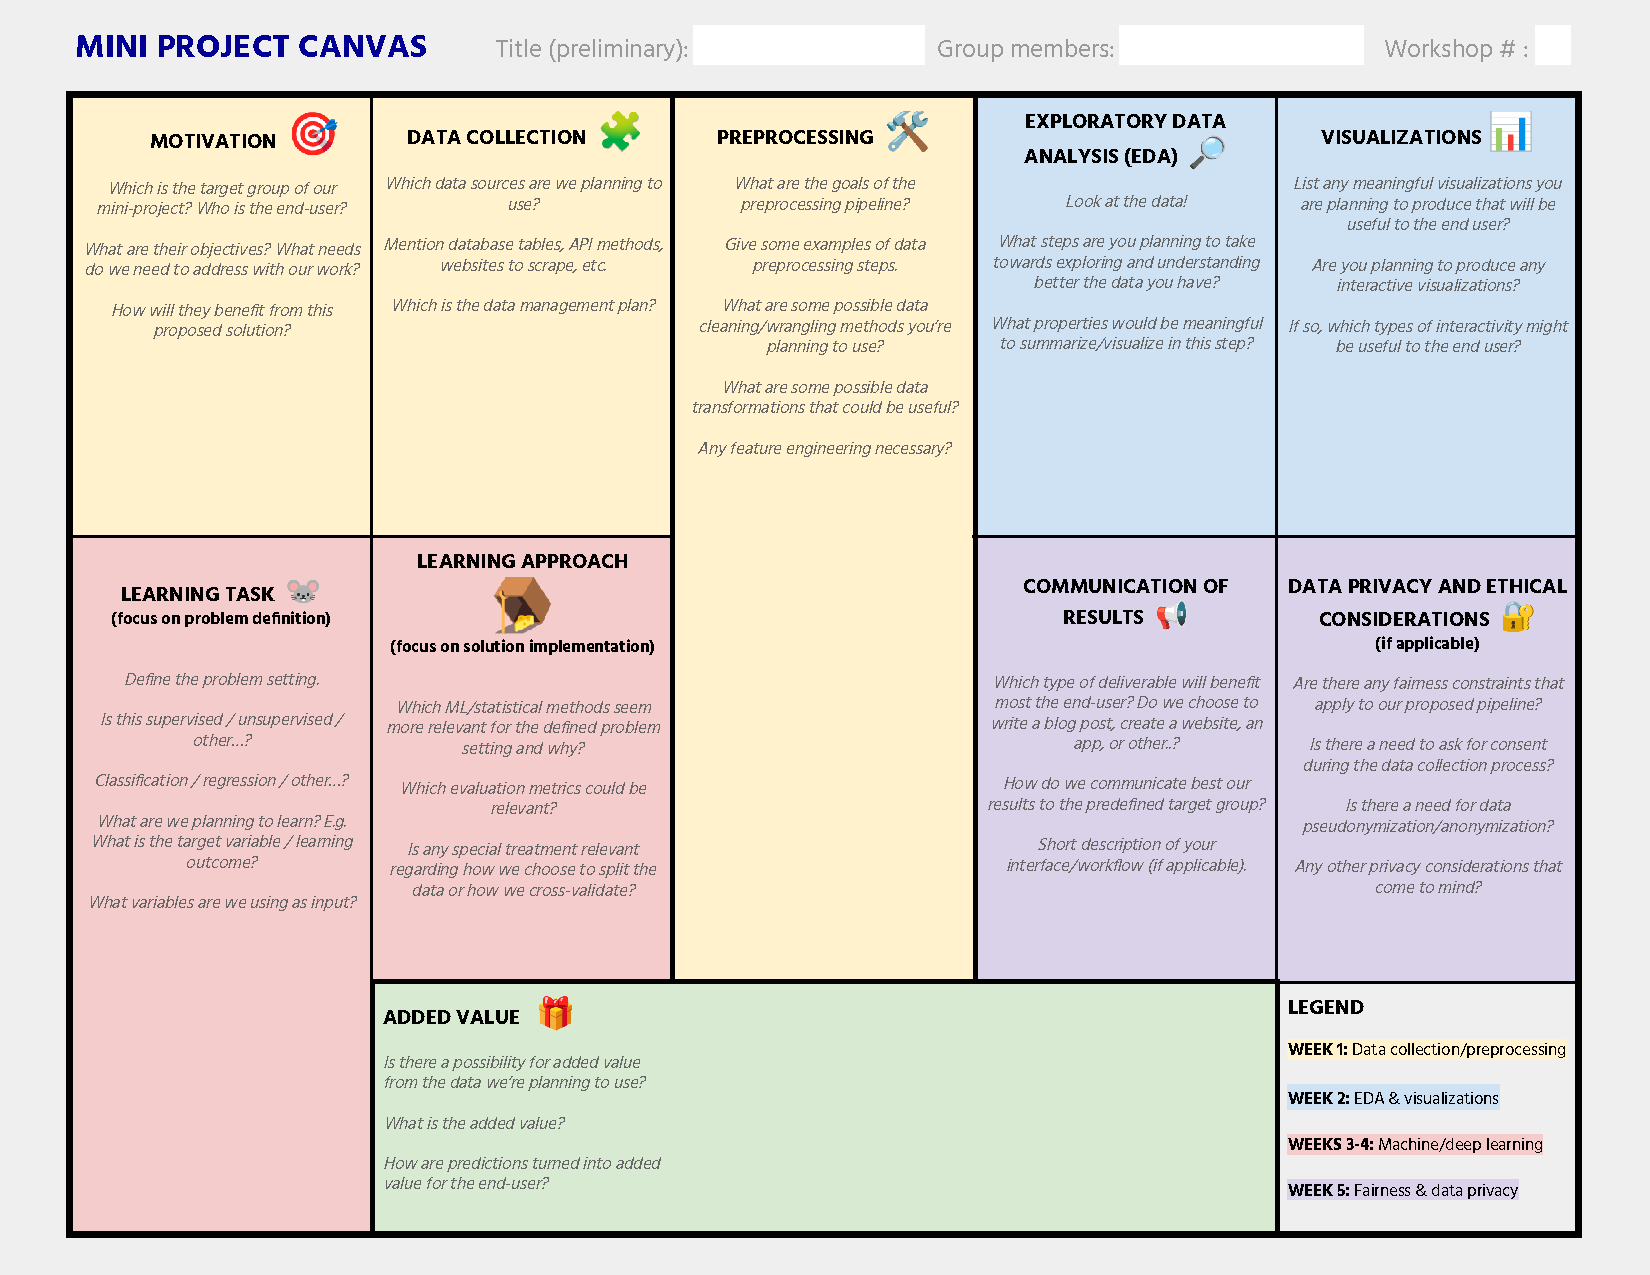
\includegraphics[width=1\textwidth]{./mini_project_canvas.pdf}
	\caption{Canvas used for project planning.}
	\label{fig1}
\end{figure}

% ---- Data Collection and Preprocessing ----
\section{Data Collection and Preprocessing}
\begin{itemize}
	\item Where is data used from?
	\item How is data stored?
	\item What kind of data is used?
	\item How is data accessed?
	\item What kind of preprocessing is done?

	Firstly, we gathered historical spot price data for Finland from the website https://porssisahko.net/tilastot. Additionally, we collected weather data from the Finnish Meteorological Institute (https://www.ilmatieteenlaitos.fi/avoin-data/) and electricity consumption and production data from Fingrid's open data platform (https://data.fingrid.fi/en/datasets/124 and https://data.fingrid.fi/en/datasets/192, respectively). All datasets were in Excel format and were downloaded using specific start and end dates as parameters. The data was then imported into a Jupyter notebook using Python, where we created a Pandas DataFrame for each dataset. We then proceeded to preprocess the data to ensure a consistent structure across all datasets.

Preprocessing began with the spot price data, which consisted of two columns: 'Aika' (time) and 'Hinta (snt/kWh)' (price). We adjusted the time column so that prices were aligned with every even hour, and applied this format to the other datasets as well. In the weather data, the year, month, day, and hour were originally in separate columns, so we combined them into a single datetime object. Since the observations were already recorded hourly, no further significant modifications were needed. Different elements of the weather data, such as mean temperature, were stored in separate columns, similar to the structure of the electricity price data.

The electricity consumption and production data, retrieved from the same open data platform, had similar structures. Both datasets included two time-related columns—'startTime' and 'endTime'—along with a column for production or consumption values. We consolidated the two time columns into one, following the same approach used for the weather data. Additionally, the time column still contained extraneous characters, which were cleaned up, and the values were converted into datetime objects.

The main difference between the production and consumption datasets was the frequency of observations: production data was recorded every three minutes, while consumption data was recorded hourly. To standardize the data, we calculated the hourly average for the production data to match the required format.

Once all the datasets were in the correct format, we merged them into a comprehensive dataframe. We then performed imputation, replacing any missing values with the column medians. Finally, we added one more input variable: a boolean variable indicating whether the date of an observation fell on a public holiday. The public holiday dates were sourced from the website https://www.officeholidays.com/countries/finland/2021.

All the data collection and preprocessing described above was carried out in a single Jupyter notebook. In addition, we created three separate Jupyter notebooks, each dedicated to handling one API. These APIs were used to fetch weather, electricity consumption, and electricity production forecasts for the upcoming days. The API used for the weather forecast is available at https://api.open-meteo.com/v1/forecast, and the data retrieved required no significant preprocessing. Electricity consumption and production predictions were collected via APIs available on the same Fingrid open data platform as the historical data. Since the prediction data had a structure very similar to the historical data, we were able to reuse the preprocessing methods to bring the predictions into the desired format.
\end{itemize}

% ---- EDA and Visualizations ----
\section{Exploratory Data Analysis and Visualizations}
\begin{itemize}
	\item What kind of EDA was done?
	\item How was the data visualized?
	\item What kind of findings were obtained?
\end{itemize}

% ---- Learning ----
\section{Learning to Predict Electricity Spot prices}
\begin{itemize}
	\item What kind of approaches were tried?
	\item What kind of observations were made during this process?
	\item What approach was used in the end? Why? How did we end up to it?
\end{itemize}

% ---- Communciation of Results ----
\section{Communication of Results}
\begin{itemize}
	\item Webpage, how?
	\item What kind of user interface is used?
	\item What does the webpage do? What can the user do?
\end{itemize}

% ---- Summary ----
\section{Summary}
\begin{itemize}
	\item Predicting electricity spot prices is difficult
	\item Nevertheless, a decent method was found for the used input variables
	\item We learned alot, maybe list here someof the thigs that we discussed
	\item What could be done better / future continuation topics
\end{itemize}


% ----------------------------------------------------------------
\iffalse
\begin{figure}[htb]
\centering
\includegraphics[width=.5\textwidth]{./largestEigenvalue.eps}
\caption{Suurimman ominaisarvon approksimaatiovirheen itseisarvo $i$:n funktiona.}
\label{fig1}
\end{figure}
\fi

\end{document}
